\documentclass[../main.tex]{subfiles}

\graphicspath{{../images/}}

\begin{document}

\section{Lecture 1/16/24}
% vertical bar
\hrule \vspace{10px}

\subsection*{Chapter 1: Crystal Structure}
\paragraph{Ideal crystal is constructed by the infinite repetition of identical structural groups of
atoms.} A group is called the basis. Detecting crystal structure started with x-rays due to the
wavelength of the x-ray ($\approx 1$ angstrom) being comparable to the interatomic spacing in a crystal.

\paragraph{What is a \emph{lattice}?}

2D Bravais Lattices \href{https://en.wikipedia.org/wiki/Bravais_lattice}{Wikipedia}
The gamous graphene has a hexagonal (honeycomb structure) like lattice, but it does not have the 
center atom from the true hexagonal lattice. The primitive of this lattice is made of up two atoms
than can be translated to form the lattice. Thus graphene is like a diatomic crystal. 

\paragraph{3D Bravais Lattices} There are 14 Bravais lattices in 3D. In both 2D and 3D, the primitive
cells that make up the lattice must fill the least amount of space and have no `holes' or `extras' left
over. The 2 most common lattices now are the Primitive Hexagonal for its symmetry and the Body
Centered Cubic (BCC) which is the lattice of Silicon, the most important material today. 

\paragraph{Example Structures}
% figure of nacl.png and cscl.png
\begin{figure}[ht]
    \centering
    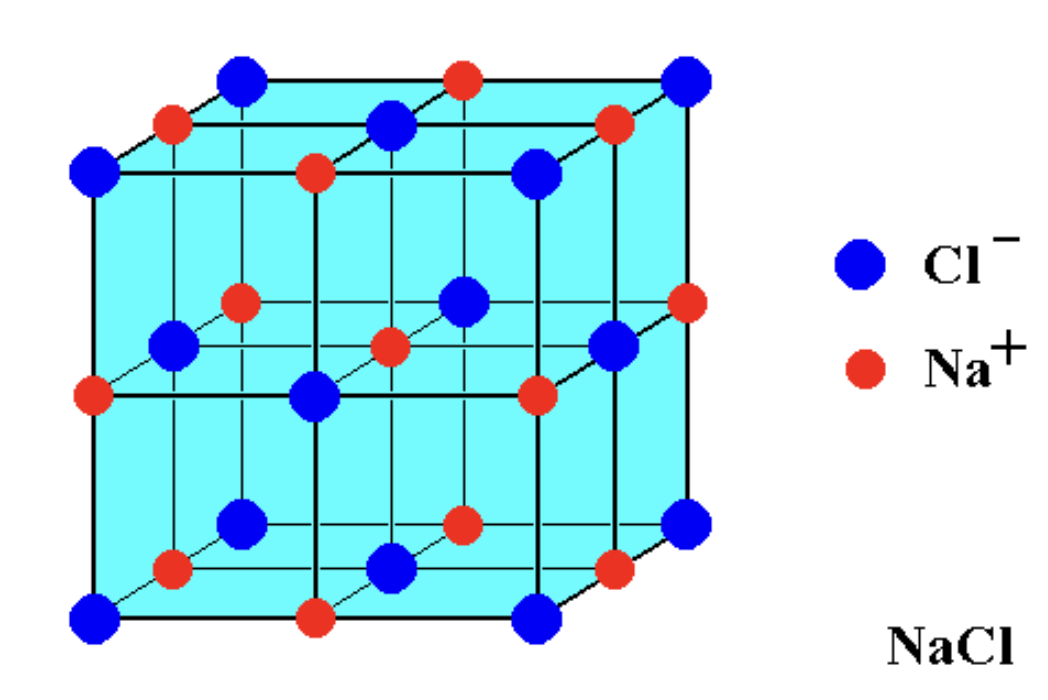
\includegraphics[scale=0.3]{nacl.png}
    \caption{Sodium Chloride Structure (FCC)}
    \label{fig:1.1}
\end{figure}

The lattice of Sodium Chloride is FCC as shown in Figure \ref{fig:1.1}

\begin{figure}[ht]
    \centering
    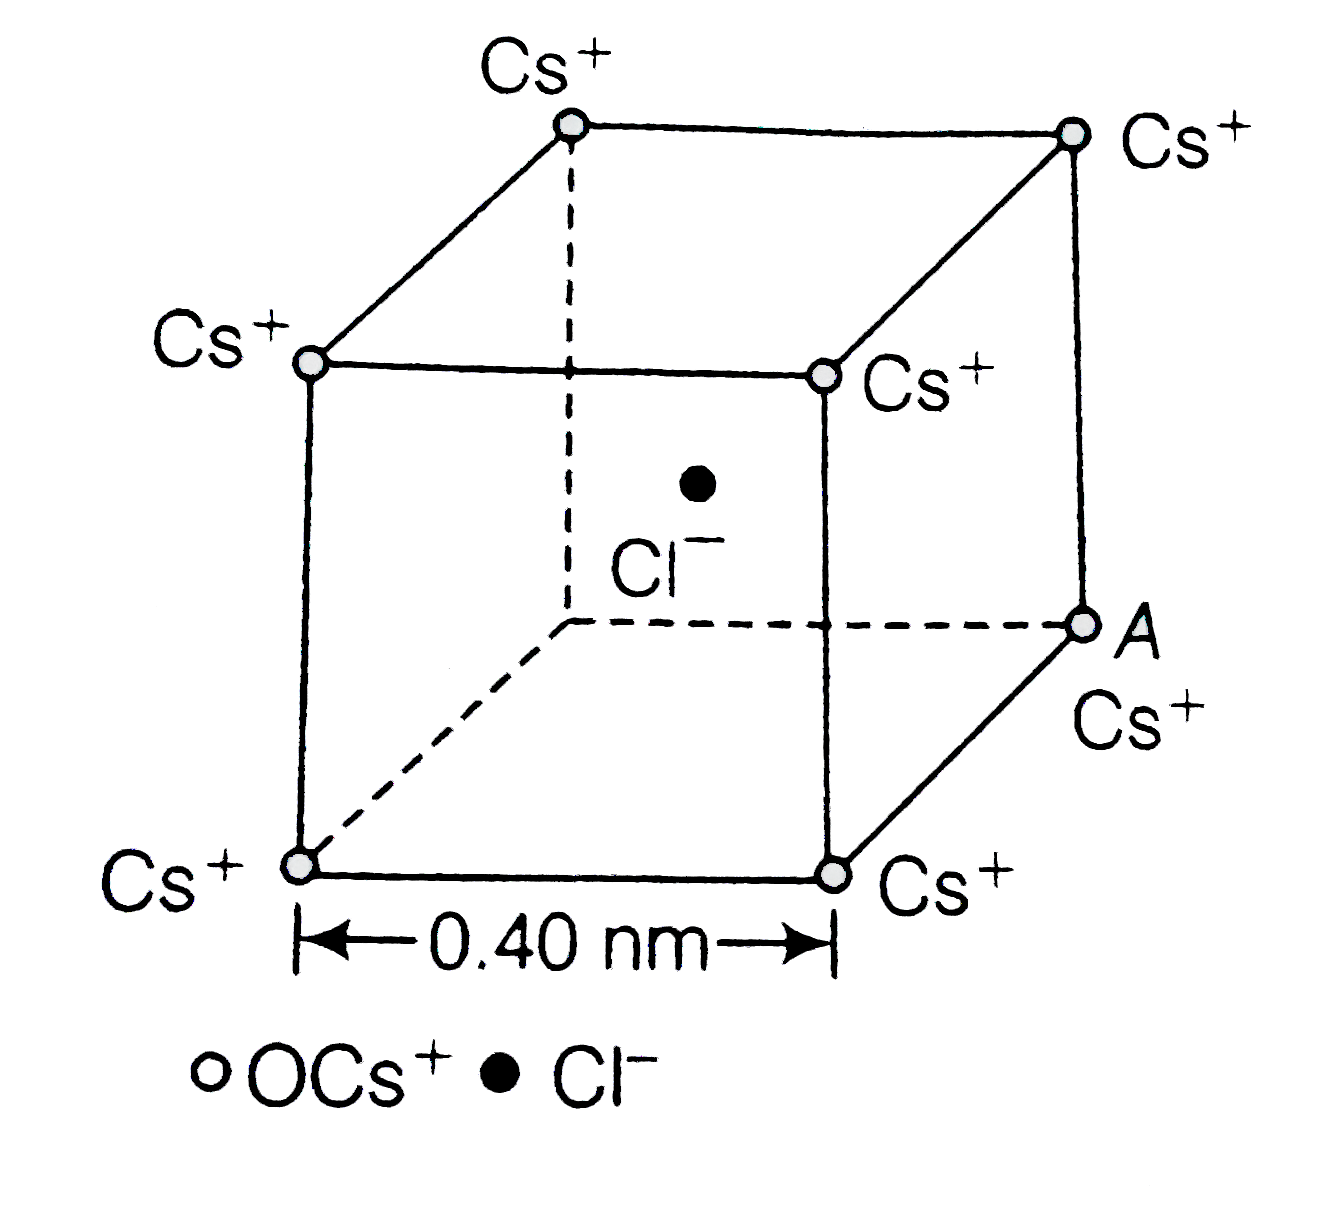
\includegraphics[width=0.3\linewidth]{cecl.png}
    \caption{Cesium Chloride Structure (SC)}
    \label{fig:1.2}
\end{figure}

Figure \ref{fig:1.2} shows the lattice of Cesium Chloride which is SC.

\newpage
\section{Lecture 1/18}
\hrule \vspace{10px}

\subsection*{Chapter 2: Wave Diffraction and the Reciprocal Lattice}

% figure of bragg.png
\begin{figure}[ht]
    \centering
    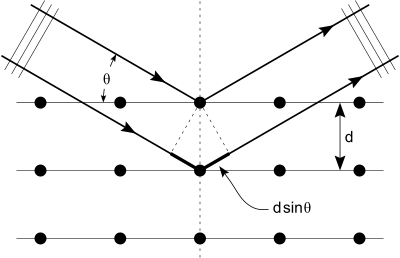
\includegraphics[width=0.4\linewidth]{bragg.png}
    \caption{Bragg's Law}
    \label{fig:2.1}
\end{figure}

\paragraph{Scattering and Bragg's Law}

When two beams of same phase meet, they constructively interfere. When they are out of phase, they
destructively interfere. The location of constructive interference, or path difference, is shown
by the bold lines in Figure \ref{fig:2.1}. The path difference is
\begin{align*}
    2d \sin \theta = n \lambda
\end{align*}
known as Bragg's Law which is only valid for $\lambda \leq 2d$. In reality each lattice plane will
reflect about $10^{-3} \sim 10^{-5}$ of the incident beam. Thus only about $10^3 \sim 10^5$ planes
contribute to the diffraction. The periodicity of the lattice leads to a periodic observable\dots

\emph{aside:} The electron wavefunction is not observable---$\psi$ is a complex number, but the
electron density, $\psi^* \psi$, is observable. Read about the quantized Hall effect (Queen):) and
Superconductivity (King).

\begin{align*}
    \psi(x + T) = \psi(x) e^{i\theta}
    n(x + T) = n(x)
\end{align*}

\paragraph{Fourier Transform} The discrete Fourier transfrom is useful for periodic functions.

\begin{align*}
    n(x) &= \sum_{P \geq 0} \qt[C_p \cos(\frac{2\pi}{a}x) + S_p \sin(\frac{2\pi}{a}x)] \\
    &= \sum_{p} n_p e^{i\frac{2\pi}{a}px}
\end{align*}
or in vector notation
\begin{align*}
    n(\vb{r}) = \sum_{\vb{G}} n_G e^{i\vb{G} \vdot \vb{r}}
\end{align*}
Since $n(x)$ is real, there is a symmetry of the complex conjugate
\begin{align*}
    n_p = n_{-p}^*
\end{align*}

\paragraph{Inverse Fourier Transform}
\begin{align*}
    n_p = \frac{1}{a} \int_0^a n(x) e^{-i\frac{2\pi}{a}px} \dd{x}
\end{align*}
and in vector notation
\begin{align*}
    n_G = \frac{1}{V} \int_{cell} n(\vb{r}) e^{-i\vb{G} \vdot \vb{r}} \dd{V}
\end{align*}

\paragraph{Reciprocal Space Vectors}

The basis vectors of the reciprocal lattice are
\begin{align*}
    \vb{b}_1 = 2\pi \frac{\vb{a}_2 \cross \vb{a}_3}{\vb{a}_1 \vdot (\vb{a}_2 \cross \vb{a}_3)};
    \quad \vb{b}_2 = 2\pi \frac{\vb{a}_3 \cross \vb{a}_1}{\vb{a}_1 \vdot (\vb{a}_2 \cross \vb{a}_3)};
    \quad \vb{b}_3 = 2\pi \frac{\vb{a}_1 \cross \vb{a}_2}{\vb{a}_1 \vdot (\vb{a}_2 \cross \vb{a}_3)}
\end{align*}
where the denominator is the volume of the unit cell (parallelpiped)
$\vb{a}_1 \vdot (\vb{a}_2 \cross \vb{a}_3) = V_c$.

Taking the dot product of a primitive vector with a reciprocal lattice vector gives
\begin{align*}
    \vb{a}_i \vdot \vb{b}_j = 2\pi \delta_{ij}
\end{align*}
where the Kronecker delta tells us that the dot product is either $2\pi$ or $0$. With this we can
write the $\vb{G}$ vector as a linear combination of the reciprocal lattice vectors
\begin{align*}
    \vb{G} = v_1\vb{b}_1 + v_2\vb{b}_2 + v_3\vb{b}_3
\end{align*}
we can also show that
\begin{align*}
    n(\vb{r} + \vb{T}) = n(\vb{r})
\end{align*}
which means that this is invariant under tranlsations.

\paragraph{Scattering amplitude}
\begin{align*}
    F = \int \dd{\vb{r}} n(\vb{r}) e^{i\vb{k} \vdot \vb{r}} e^{-i\vb{k}' \vdot \vb{r}}
\end{align*}
where $\abs{\vb{k}} = \abs{\vb{k}'}$. In vector notation
\begin{align*}
    F &= \int \dd{\vb{r}} \sum_{\vb{G}} n_G e^{i(\vb{G} - \vb{r}')} e^{-i\Delta\vb{k} \vdot \vb{r}} \\
    &= \sum_{\vb{G}} n_G \int \dd{\vb{r}} e^{i(\vb{G} - \Delta\vb{k}') \vdot \vb{r}} \\
\end{align*}
where $\Delta\vb{k} = -(\vb{k} - \vb{k}')$. When $\vb{G} = \Delta\vb{k}$ we can rewrite to
\begin{align*}
    \vb{k} + \Delta\vb{k} = \vb{k}'
\end{align*}
in absolute value
\begin{align*}
    \abs{\vb{k} + \Delta\vb{k}} = \abs{\vb{k}'} \rightarrow
    \abs{\vb{k} + \Delta\vb{k}} = \abs{\vb{k}} \rightarrow
    \abs{\vb{k} + \vb{G}} = \abs{\vb{k}}
\end{align*}
and
\begin{align*}
    (\vb{k} + \vb{G}) \vdot (\vb{k} + \vb{G}) = \vb{k} \vdot \vb{k} \rightarrow
    2\vb{k} \vdot \vb{G} + \vb{G}^2 = 0
\end{align*}
For the 1D crystal $G = 2\pi / a$. Since $\vb{k} \vdot \vb{G} = 2\pi/\lambda \vb{G} \sin\theta$
and $2\vb{k} \vdot \vb{G} = \vb{G}^2$
We get
\begin{align*}
    2 \vdot \frac{2\pi}{\lambda} G \sin\theta &= \vb{G}^2 \\
    \rightarrow \frac{4\pi}{\lambda} \sin\theta &= G 
\end{align*}
since $G = 2\pi / a$ we get Bragg's Law
\begin{align*}
    2d \sin\theta = n\lambda
\end{align*}
For the SC the reciprocal lattice is SC, but for BCC, the reciprocal lattice is different\dots

\newpage
\section{Lecture 1/23/24}
% vertical bar
\hrule \vspace{10px}

\subsection*{Chapter 2: cont'd}

\paragraph{Wigner-Seitz primitive cell:} How to create the most symmetric primitive cell.

% figure of pcell.png
\begin{figure}[ht]
    \centering
    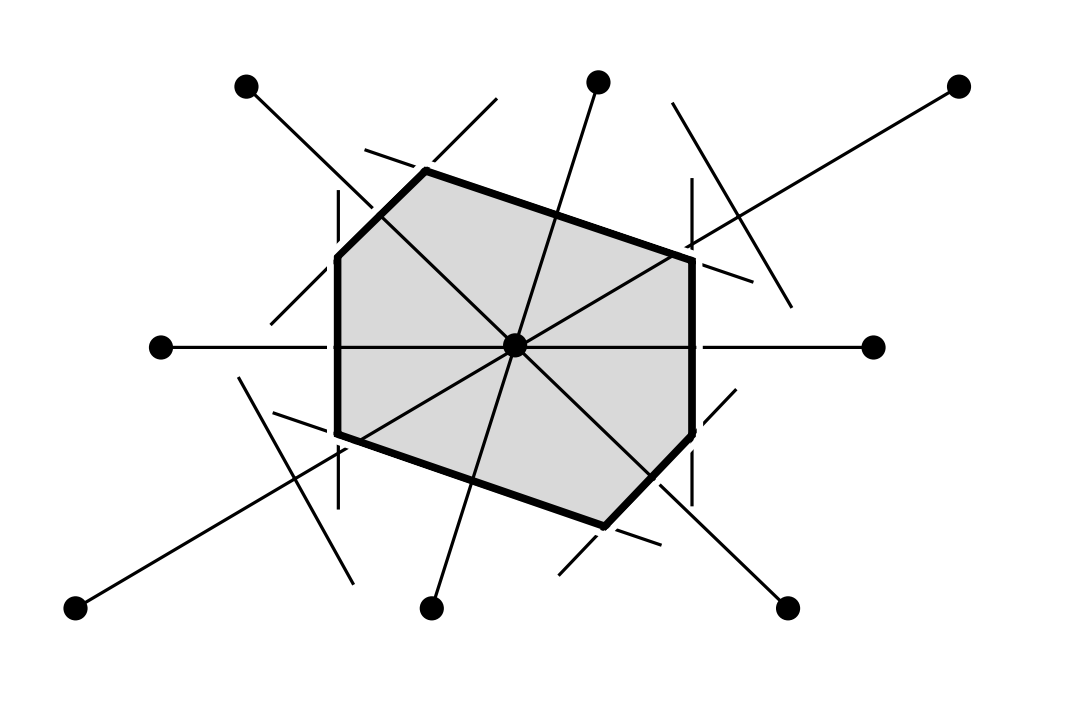
\includegraphics[width=0.4\linewidth]{pcell.png}
    \caption{Wigner-Seitz Primitive Cell}
    \label{fig:3.1}
\end{figure}
Steps: Connect a given lattice point to all nearby lattice points. Bisect all lines. The area 
enclosed by the bisectors is the Wigner-Seitz primitive cell as shown in Figure \ref{fig:3.1}.

\paragraph{Reciprocal Lattice of SC} The lattice vectors (primitive translation vectors) are
\begin{align*}
    \vb{a}_1 = a\vu{x}, \quad \vb{a}_2 = a\vu{y}, \quad \vb{a}_3 = a\vu{z}
\end{align*}
the reciprocal lattice vectors using the formula from last lecture are
\begin{align*}
    \vb{b}_1 = 2\pi \frac{\vb{a}_2 \cross \vb{a}_3}{V_c} = \frac{2\pi}{a}\vu{x}, \quad
    \vb{b}_2 = \frac{2\pi}{a}\vu{y}, \quad \vb{b}_3 = \frac{2\pi}{a}\vu{z}
\end{align*}

\paragraph{Reciprocal Lattice of BCC} The lattice vectors are
\begin{align*}
    \vb{a}_1 = \frac{a}{2}(-\vu{x} + \vu{y} + \vu{z}), \quad
    \vb{a}_2 = \frac{a}{2}(\vu{x} - \vu{y} + \vu{z}), \quad
    \vb{a}_3 = \frac{a}{2}(\vu{x} + \vu{y} - \vu{z})
\end{align*}
and the reciprocal lattice vectors are
\begin{align*}
    \vb{b}_1 = \frac{2\pi}{a}(\vu{y} + \vu{z}), \quad
    \vb{b}_2 = \frac{2\pi}{a}(\vu{z} + \vu{x}), \quad
    \vb{b}_3 = \frac{2\pi}{a}(\vu{x} + \vu{y})
\end{align*}

\paragraph{Reciprocal Lattice of FCC} The lattice vectors are
\begin{align*}
    \vb{a}_1 = \frac{a}{2}(\vu{y} + \vu{z}), \quad
    \vb{a}_2 = \frac{a}{2}(\vu{x} + \vu{z}), \quad
    \vb{a}_3 = \frac{a}{2}(\vu{x} + \vu{y})
\end{align*}
which is the same as the reciprocal space of BCC. Thus, the reciprocal lattice of FCC is BCC!

\paragraph{Brillouin Zone} The first Brillouin zone is the Wigner-Seitz primitive cell of the
reciprocal lattice.

\subsection*{Chapter 3: Crystal Binding and Elastic Constants}

We are mostly interested in the E\&M interaction between atoms on the energy scale of eV (e.g. the
band gap of silicon is 1.2 eV). 

\paragraph{There are 4 main types of bonds:}

\subparagraph*{Metallic Bond} Bonds between metals have weakly bound valence electrons. Hence the
electrons move freely around like a fluid. This is why metals are good conductors.

\subparagraph*{Ionic Bond} Bonds between metals and non-metals (e.g. NaCl). The opposing charges
attract each other where the electrons form full shells and hence less conductivity.

\subparagraph*{Covalent Bond} Bonds between non-metals (e.g. Si). The atomic orbitals defined by
QM describes the bonds through the hybridization of the orbital wavefunctions (e.g. $sp^3$ in
diamond). This is a very difficult problem to solve.

\subparagraph*{Van der Waals interaction} Inert gases... e.g. He is interesting as it is a liquid at
very low temperatures, and it is a boson (He-4 superfluid) and fermion (He-3) depending on the
number of neutrons. 

\subparagraph*{Hydrogen Bonding} is very important in biology, but not in solid state physics.

\subsection*{Van der Waals interaction}

Two types of energy to consider:
\begin{itemize}
\item Cohesive energy: Energy required to separate bound atoms. The cohesive energy of a solid
is the sum of the cohesive energies of the bonds. 
\item Ionization energy: Energy required to remove an electron from an atom.
\end{itemize}

The ionization energy is larger because the Van der Waals interaction is a weaker bond. Given two
inert gas atoms, there is no dipole or charge distribution contributing to the interactions between
the atoms. In QM, there is no zero point energy, so we have to consider the atoms to not be perfect,
but rather vibrate around a mean position. This is a dipole-dipole interaction. 

\paragraph{dipole-dipole }Given two electrons spaced by a distance $R$ in a 1D lattice, one atom
fluxuates by $x_2$ and the other by $x_1$. The Hamiltonian of the unpertubed system is
\begin{align*}
    H_o = \frac{p_1^2}{2m} + \frac{p_2^2}{2m} + \frac{1}{2} C x_1^2 + \frac{1}{2} C x_2^2
\end{align*}
The Coulomb interaction:
\begin{align*}
    H_1 = \frac{e^2}{R} + \frac{e^2}{R + x_1 - x_2} - \frac{e^2}{R + x_1} - \frac{e^2}{R - x_2}
\end{align*}
Using Taylor expansion (2nd order) for small $x_1$ and $x_2$ we get
\begin{align*}
    H_1 = -\frac{2e^2}{R^3} x_1 x_2
\end{align*}
Since this has 2 degrees of freedom, we have a 2x2 matrix with 2 eigenvalues diagonlized by the
normal mode transform. This results in 2 Canconical Modes:
\begin{align*}
    x_s = \frac{1}{\sqrt{2}}(x_1 + x_2) \quad x_a = \frac{1}{\sqrt{2}}(x_1 - x_2)
\end{align*}
THe total Hamiltonian is
\begin{align*}
    H &= \frac{1}{2m} \qt[\frac{1}{2}(p_s + p_a)^2] + \frac{1}{2m}\qt[\frac{1}{2}(p_s - p_a)^2]
    - 2 \frac{e^2}{R^3} \cdot \frac{1}{2} (x_s^2 - x_a^2) + \frac{1}{2} cx_1^2 + \frac{1}{2} cx_2^2\\
    &= \qt[\frac{p_s}{2m} + \frac{1}{2} \qt(c - \frac{2e^2}{R^3})x_s^2] +
    \qt[\frac{p_a}{2m} + \frac{1}{2} \qt(c + \frac{2e^2}{R^3})x_a^2]
\end{align*}

\pagebreak
\section{Lecture 1/25/24}
\hrule \vspace{10px}

\subsection*{Chapter 3: cont'd}

The momenta of the harmonic oscillators from last time are also in the ofmr 2 modes:
\begin{align*}
    p_s = \frac{1}{\sqrt{2}}(p_1 + p_2) \quad p_a = \frac{1}{\sqrt{2}}(p_1 - p_2)
\end{align*}
The matrix form
\begin{align*}
    \begin{pmatrix}
        E_o & 0 \\
        0 & E_o
    \end{pmatrix} \mqty(a \\ b)
    = \hbar \omega \mqty(a \\ b)
\end{align*}
\begin{align*}
    \begin{vmatrix}
        E_o - \hbar \omega & \Delta \\
        \Delta & E_o - \hbar \omega
    \end{vmatrix}
    = 0
\end{align*}
solving for the eigenstates
\begin{align*}
    \frac{1}{\sqrt{2}} \mqty(a \\ b), \quad \frac{1}{\sqrt{2}} \mqty(a \\ -b)
\end{align*}
The Hamiltonian of the single harmonic oscillator is
\begin{align*}
    H_o = \frac{p^2}{2m} + \frac{1}{2} m \omega^2 x^2
\end{align*}
thus we can compare the frequencies of the harmonic oscillator and the Van der Waals interaction
\begin{align*}
    \omega = \sqrt{\frac{c \pm \frac{2e^2}{R^3}}{m}}
\end{align*}
and we know the \emph{zero-point energy} $1/2 \hbar \omega$ or in this case 
\begin{align*}
    \frac{1}{2} \hbar \Delta \omega = \frac{1}{2} \hbar [\Delta \omega_s + \Delta \omega_a]
\end{align*}
From the uncoupled sum and using Taylor expansion
\begin{align*}
    \omega = \omega_o \qt[1 \pm \frac{1}{2} \qt(\frac{2e^2}{R^3c})
    \pm \frac{1}{8} \qt(\frac{2e^2}{R^3c})^2 + \dots]
\end{align*}
thus we ge the interaction energy
\begin{align*}
    \Delta U = \frac{1}{2} \hbar (\Delta \omega_s + \Delta \omega_a)
    = \frac{\hbar\omega_o}{2} \qt[\frac{e^4}{c^2 R^6}] = -\frac{A}{R^6}
\end{align*}
where the minus sign indicates an attractive force. We would expect the atoms to collapse, but
this is not the case due to the Pauli exclusion principle (electrons cannot occupy the same state).

\subsubsection*{Pauli exclusion principle}

As the atoms get closer, there is an overlap of the wavefunctions. If the wavefunctions are
symmetric, the spin states must be anti-symmetric. Therefore anti-symmetric wavefunctions have
symmetric spin states. This repulsive force from the Pauli exclusion principle is typically
found empirically $\propto \frac{1}{R^{12}}$. Therefore the total potential is
\begin{align*}
    U(R) = 4 \epsilon \qt[\qt(\frac{\sigma}{R})^{12} - \qt(\frac{\sigma}{R})^{6}]
\end{align*}
AKA the Lennard-Jones potential. We could find the equilibrium distance by minimizing the
potential $\dv{U}{R} = 0$. This is fine for inert gases that are spherical, but other molecules are
depend on more than the scalar distance $R$. This decays faster than the scale of Coulombs Law
$\propto \frac{1}{R^2}$. The total energy for a crystal is
\begin{align*}
    E = \frac{1}{2} N (4\epsilon) \qt[
        \sum_j ' \qt(\frac{\sigma}{P_{ij}R})^{12} - \sum_j ' \qt(\frac{\sigma}{P_{ij}R})^{6}
    ]
\end{align*}
where the prime indicates that the sum is over the nearest neighbors. The fcc lattice
\begin{align*}
    \sum_j' \qt(\frac{1}{P_{ij}})^{12} = 12.13188; \qquad \sum_j' \qt(\frac{1}{P_{ij}})^6 = 14.45392
\end{align*}
for the 12 nearest neighbors. Solving for the minimum energy $\dv{U}{R} = 0$ we get 
\begin{align*}
    R_o / \sigma = 1.09
\end{align*}

\subsubsection*{Ionic Crystal}

The Coulomb interaction: 
\begin{align*}
    \pm \frac{q^2}{r_{ij}}
\end{align*}
The short-term interaction 
\begin{align*}
    \lambda e^{-r_{ij}/\rho}
\end{align*}
thus the potential is
\begin{align*}
    U_{ij} = \lambda e^{-r_{ij}/\rho} \pm \frac{q^2}{r_{ij}}
\end{align*}
where at one site (one ion)
\begin{align*}
    U_i = \sum_j' U_{ij}
\end{align*}
and the total energy is
\begin{align*}
    U = N U_i
\end{align*}
For N molecules
\begin{align*}
    U_{ij} = \begin{cases}
        \lambda e^{-r_{ij}/\rho} - \frac{q^2}{r_{ij}} & \text{nearest neighbor} \\
        \pm \frac{q^2}{r_{ij}} & \text{otherwise}
    \end{cases}
\end{align*}
and the total energy is
\begin{align*}
    U_{tot} = N \qt[z e^{-R/\rho} - \alpha \frac{q^2}{R}] \qquad \alpha = \sum_j' \frac{\pm}{p_{ij}}
\end{align*}
where $z$ is the number of nearest neighbors, and $\alpha$ is the Madelung constant. From this we
can find the lattice constant by using
\begin{align*}
    \dv{U}{R} = 0 \rightarrow R_o^2 e^{-R_o/\rho} = \alpha \rho \frac{q^2}{z\lambda}
\end{align*}
solving for $R_o$ and putting into the total energy equation we get
\begin{align*}
    U_{tot} = -\frac{N\alpha q^2}{R_o} (1 - \frac{\rho}{R_o}) 
\end{align*}
where we have a special term
\begin{align*}
    -\frac{N\alpha q^2}{R_o}
\end{align*}
known as the `Madelung Energy'.

\pagebreak
\section{Lecture 1/30/24}
\hrule \vspace{10px}

\subsection*{Chapter 3: Bonds Bonds and Bonds}
From last time:
\begin{align*}
    U_{ij} = \begin{cases}
        \lambda e^{-R/\rho} - \frac{q^2}{R} & \text{nearest neighbor} \\
        \pm \frac{q^2}{p_ijR} & \text{otherwise}
    \end{cases}
\end{align*}
where $p_{ij}R = r_{ij}$ and the total energy (sum) is
\begin{align*}
    U_{tot} = N \qt[z e^{-R/\rho} - \alpha \frac{q^2}{R}]
\end{align*}
where $z$ is the number of nearest neighbors, $N$ is the total ions, and $\alpha$ is the Madelung
constant:
\begin{align*}
    \alpha = \sum_j' \frac{\pm}{p_{ij}}
\end{align*}
At the equilibrium seperation
\begin{align*}
    \dv{U}{R} = 0 \rightarrow R_o^2 e^{-R_o/\rho} = \alpha \rho \frac{q^2}{z\lambda}
\end{align*}
$R_o$ is the equilibrium seperation (position). Substituting this back into the total energy we get
the empirical formal for the equilibrium energy (ground state):
\begin{align*}
    U_{tot} = -\frac{N\alpha q^2}{R_o} \qt(1 - \frac{\rho}{R_o})
\end{align*} 
where the first term outside the parenthesis is the Madelung energy
\begin{align*}
    -\frac{N\alpha q^2}{R_o}
\end{align*}
\paragraph{The Evaluation of Madelung Constant}
\begin{figure}[ht]
    \centering
    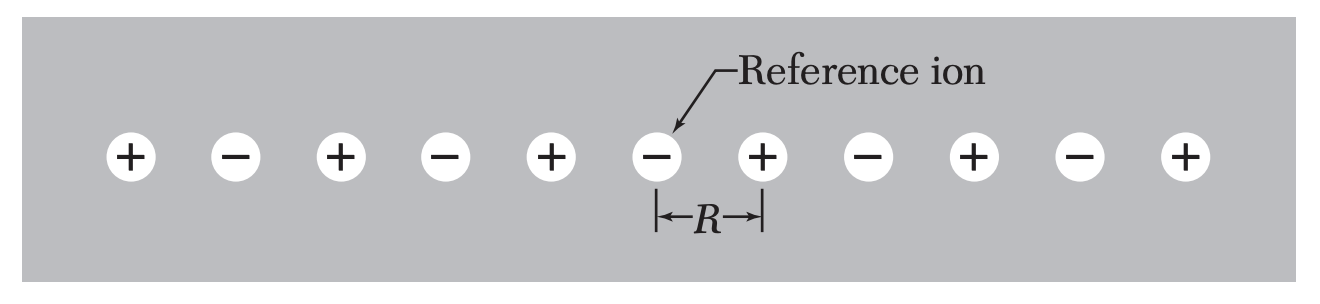
\includegraphics[width=0.4\linewidth]{ionline.png}
    \caption{Line of ions with alternating charges}
    \label{fig:4.1}
\end{figure}
Letting $R$ denote the distance between the ions, we can write the Madelung constant for the 1D line
of ions with alternating charges as.
\begin{align*}
    \frac{\alpha}{R} &= 2\qt[
        \frac{1}{R} - \frac{1}{2R} + \frac{1}{3R + \dots}
    ] \\
    &= \frac{2}{R} \qt[1 - \frac{1}{2} +...] \\
    \alpha &= 2 \ln{2} 
\end{align*}
Remember these numbers
\begin{itemize}
    \item Bohr radius $a_o = 0.529 {A}$
    \item fine structure constant $\alpha = \frac{e^2}{\hbar c} = \frac{1}{137}$
\end{itemize}
For the covalent bond, we have to use QM because the electron distribution is homogenous like
a sea of electrons. Sometimes we think of this as a homogenous electron gas. This is a very
difficult problem to solve. So we move on to the Hydrogen bond. This is a very weak bond typically
at the scale of meV--- room temperature is around 25 meV. So the bonds can break easily.

\pagebreak
\subsection*{Chatper 4: Phonons (lattice vibration)}

First starting with the 1D case: evenly spaced atoms we can take the minimum energy energy at the
atom and take the limit as it approaches zero or
\begin{align*}
    \pdv{U}{x} = 0
\end{align*}
the first term is $V \propto x^2$ so we can approximate the potential as
\begin{align*}
    U = \frac{1}{2} U'' x^2 = \frac{1}{2} c x^2
\end{align*}
where $c$ is the spring constant. So we can imagine that the atoms $(u_{s-1}, u_s, u_{s+1})$ are
connected by springs. For 2 coupled springs in series we end up with 2 eigenmodes. But we look at
each pair of atoms and sum up the forces. Using newton's second law we get the force of the $s$ atom 
\begin{align*}
    F_s = c (u_{s+1} - u_s) + c (u_{s-1} - u_s) = c [u_{s+1} + u_{s-1} - 2u_s]
\end{align*}
or as a differential equation
\begin{align*}
    M \dv[2]{u_s}{t} &= c [u_{s+1} + u_{s-1} - 2u_s] \\
    u &= u(\gamma) e^{-i\omega t} \\
    \implies -M \omega^2 u_s &= c [u_{s+1} + u_{s-1} - 2u_s]
\end{align*}
this momentum of the crystal is not conserved but the Hamiltonian can still be written as
\begin{align*}
    H(\gamma) H(\gamma + T)
\end{align*}
where we discretize the translational symmetry, so we can write the periodic part of the atom as
\begin{align*}
    u_s^k = u e^{-ik\gamma \qquad u(\gamma) = u(\gamma + T)}
\end{align*}
where $k = 2\pi/L$ is the wavevector. So we can write the $u_{s-1}$ and $u_{s+1}$ as a translation
of $u_s$:
\begin{align*}
    u_{s-1} &= u e^{-i(s-1)ka} \\
    u_{s+1} &= u e^{i(s+1)ka} \\
    u_s &= u e^{-iska}
\end{align*}
where $a$ is the lattice spacing. subbing this back in:
\begin{align*}
    -M \omega^2 &= c \qt[e^{-ika} + e^{ika} - 2] \\
    \omega^2 &= 2 \frac{c}{M} (1 - \cos(ka))
\end{align*}
using the trig identity for half angles we get 
\begin{align*}
    \omega^2 = \frac{4c}{M} \sin[2](\frac{ka}{2}) \qor
    \omega = 2\sqrt{\frac{c}{M}} \abs{\sin(\frac{ka}{2})}
\end{align*}
where $\omega = ck$ is the dispersion relation where we have boundaries at
$\pm \pi/a$ and max $2\sqrt{c/m}$. The group velocity is
\begin{align*}
    v_g = \pdv{\omega}{k}
\end{align*}
for $k \to 0$ we get the group velocity
\begin{align*}
    v_g = a \sqrt{\frac{c}{M}}
\end{align*}
we also get from the graph of $\omega$ is that the slope at the boundaries are zero. 

\pagebreak
\section{Lecture 2/1/24}
\hrule \vspace{10px}

\subsection*{Chapter 4: cont'd}
\begin{figure} [ht]
    \centering
    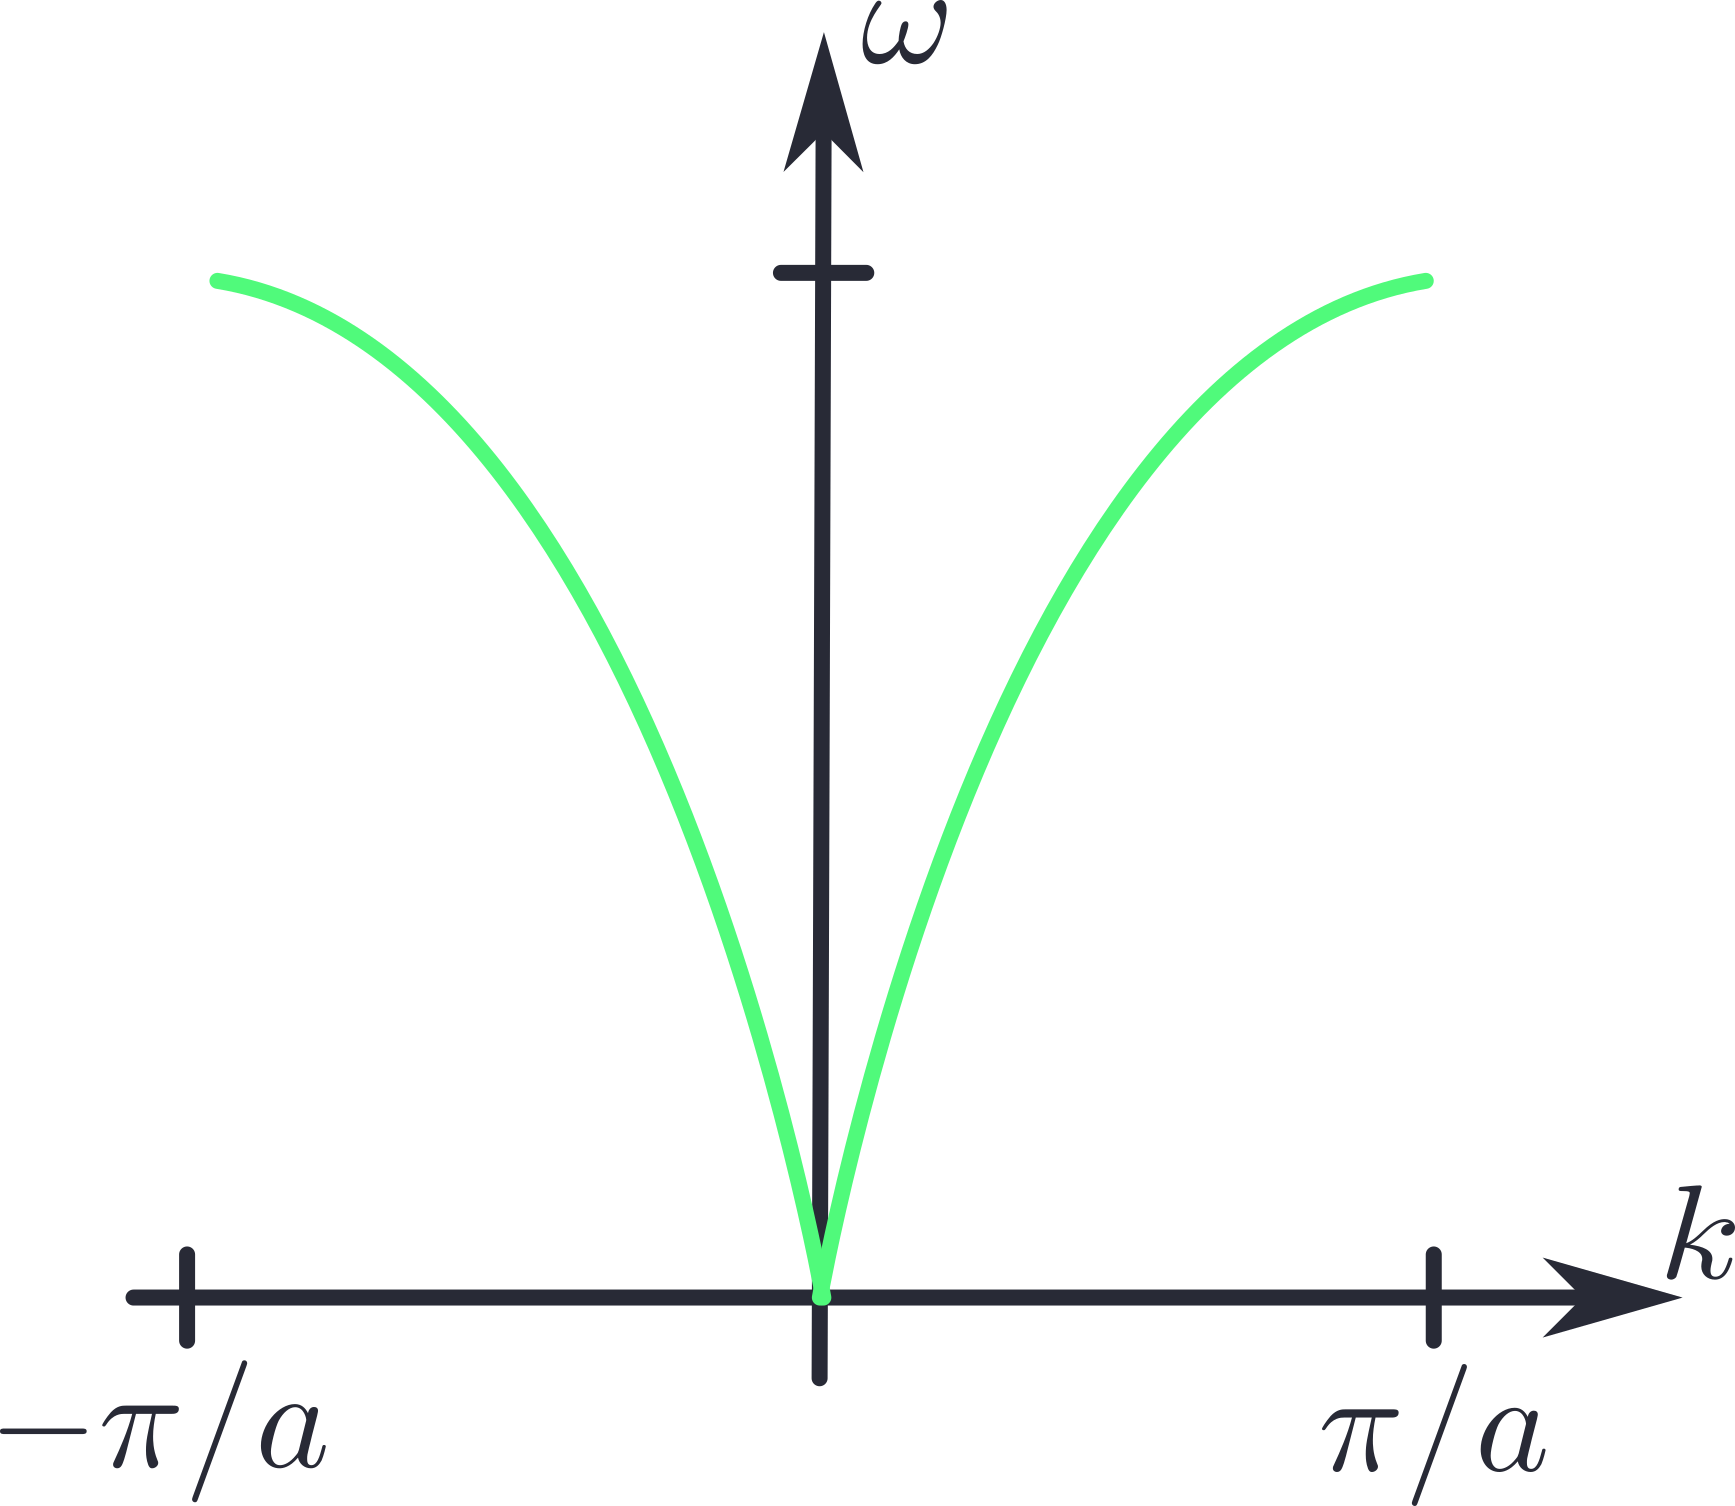
\includegraphics[width=0.4\linewidth]{phonon1.png}
    \caption{Graph of $\omega$ vs $k$}
    \label{fig:5.1}
\end{figure}

Graphing $\omega$ vs $k$ we get the graph in Figure \ref{fig:5.1}. The slope at the boundaries is
zero, and the maximum is $2\sqrt{c/M}$. But as $k \to 0$ we know that $\omega = 0$ and the energy
is also zero. We can imagine the atoms are moving in phase (oscillating in the same direction) and
amplitude. For $\omega = 2\sqrt{c/M}$ we have the atoms moving out of phase (moving in opposite of
their neighbors with equal amplitude). At this point $k = \pi/a$ the potential is
\begin{align*}
    e^{i\pi/a \cdot a} \to e^{i\pi}
\end{align*}

\begin{figure}[ht]
    \centering
    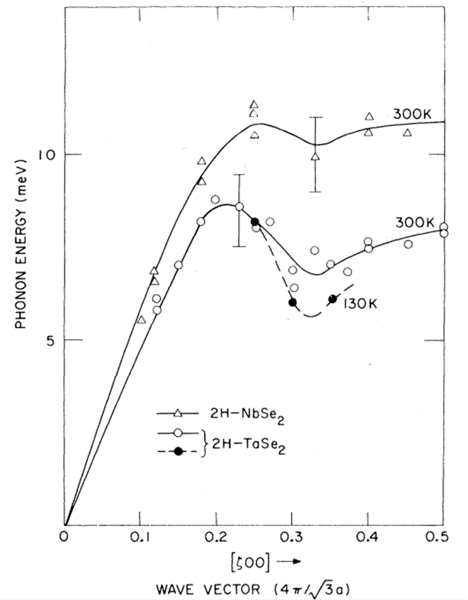
\includegraphics[width=0.4\linewidth]{phonon2.png}
    \caption{Graph of $\omega$ vs $k$ for different material and temperature}
    \label{fig:5.2}
\end{figure}
Figure \ref{fig:5.2} shows the graph of $\omega$ vs $k$ for neutron scattering observed in different
materials and temperatures. We can see that the lower temperature has a low energy mode. 

\paragraph{Aside:} For phonons in low temperature, we see a double well potential, but for high
temperatures, we see negative potential as shown in Figure \ref{fig:5.2}. 

\paragraph{Two atom per unit cell} (primitive basis) For the 1D case again:
\begin{figure}[ht]
    \centering
    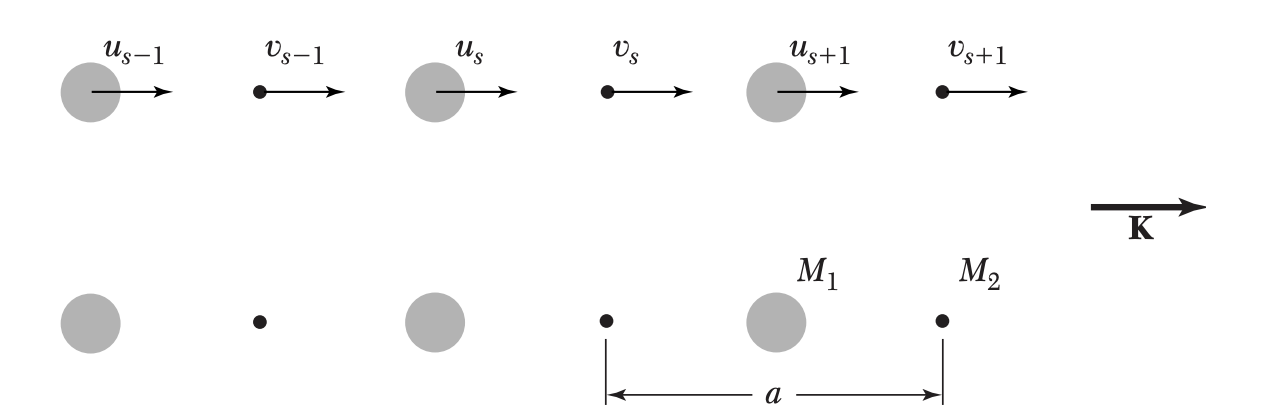
\includegraphics[width=0.8\linewidth]{2basis.png}
    \caption{Two atom per unit cell}
    \label{fig:5.3}
\end{figure}

Using newton's second law
\begin{align*}
    M_1 \ddot{u_s} &= c [v_s + v_{s-1} - 2u_s] \\
    M_2 \ddot{v_s} &= c [u_s + u_{s+1} - 2v_s]
\end{align*}
and the periodic nature of the lattice
\begin{align*}
    u_s &= u e^{iska} e^{-i\omega t} \\
    v_s &= v e^{iska} e^{-i\omega t}
\end{align*}
from substitution we get
\begin{align*}
    -M_1 \omega^2 u &= cv \qt[1 + v e^{-ika}] - 2u \\
    -M_2 \omega^2 v &= cu \qt[1 + u e^{ika}] - 2v
\end{align*}
or in matrix form
\begin{align}
    -\omega^2 \mqty(M_1 & 0 \\ 0 & M_2) \mqty(u \\ v) 
    = c \mqty(-2c & c[1 + e^{-ika}] \\ c[1 + e^{ika}] & -2c) \mqty(u \\ v)
\end{align}
to find the eigenvalues we solve the determinant of the matrix. We can only do this if the matrix is
real (hermitian: complex conjugate is the same as the original). Solving for zero
\begin{align*}
    A = \begin{vmatrix}
        -\omega^2 M_1 + 2c^2 & -c^2(1 + e^{-ika}) \\
        -c^2(1 + e^{ika}) & -\omega^2 M_2 + 2c^2
    \end{vmatrix} \mqty(u \\ v)= 0
\end{align*}
and the determinant of $A$ is
\begin{align*}
    \omega^4 M_1 M_2 - 2c^2 \omega^2 (M_1 + M_2) + 4c^4 + c^2(1 + e^{-ika})(1 + e^{ika}) &= 0 \\
    \omega^4 (M_1 M_2 - 2c^2 (M_1 + M_2) + 4c^4 - c^4[2 + 2 \cos(ka)]) &= 0
\end{align*}
for $k = 0$ we get
\begin{align*}
    M_1 M_2 w^4 - 2c[M_1 + M_2]\omega^2 = 0
\end{align*}
we get the solutions
\begin{align*}
    \omega_o &= 0 \\
    \omega_1 &= \sqrt{\frac{2c(M_1 + M_2)}{M_1 M_2}}
\end{align*}
for $k = \pi/a$ we get
\begin{align*}
    \omega^4 M_1 M_2 - 2c \omega^2(M_1 + M_2) + 4c^4 &= 0
\end{align*}
Physically, the $k=0$ mode there are two solutions, one where all basis move in the same direction,
and the other where each atom moves in the opposing direction. For $k = \pi/a$ we have a solution
where the basis pair move in the opposite direction of its neighbors. For this special case, we know
that the Brillouin zone is half the size of the original zone, so the zone folds in half. 

\paragraph{Phonon modes} For the $k=0$, in the $\omega_o = 0$ case we know that
$\lambda \to \infty$ and it is called an acoustic phonon, but for $\omega_1$ this is an optical 
phonon. This is in the order of meV around the room temperature. For energy of the phonon,
\begin{align*}
    E = \hbar \omega = pc \qand p = \hbar k
\end{align*}
Raman scattering is related to the scattering of light from the optical phonon. The wavelength of
incoming and outgoing light shift by the energy of the phonon.

\paragraph{3D Case:} $N$ atoms per unit cell. We have $3N$ branches of phonons. 3 acoustic and
$3N - 3$ optical phonon.

\newpage
\section{Lecture 2/6/24}
\hrule \vspace{10px}

\subsection*{Chapter 4: cont'd}

\paragraph*{Raman Scattering \& Infrared} (THz) $\sim$ 100 meV.
For the 3D case, we have 3 acoustic modes and $3N - 3$ optical modes. FOr the acoustic mode.
\begin{align*}
    k \to 0, \quad \omega \to 0
\end{align*}
and for the optical modes
\begin{align*}
    k \to 0, \quad \omega \to \infty
\end{align*}

\subsection*{Chapter 5: Phonon properties} 

The heat capacity is in general
\begin{align*}
    C_v = \qt(\pdv{U}{T})_v
\end{align*}
The proportionaly of heat capacity in different materials
\begin{itemize}
    \item Metal: $C_v \propto I + Q T^3$
    \item Insulator: $C_v \propto T^3$
\end{itemize}

The Energy of an $N$ particle system is $E = N k_B T$. and the heat capacity is
\begin{align*}
    C_v = \pdv{E}{T} = \omega k_B
\end{align*}
The total energy is
\begin{align*}
    U_{tot} = \sum{k, p} \hbar \omega_{k,p} \langle n_{k,p} \rangle
\end{align*}
where $\langle n_{k,p} \rangle$ is the Bose-Einstein distribution
\begin{align*}
    \langle n_\omega \rangle = \frac{1}{\exp(\frac{\hbar \omega}{k_B T}) - 1}
\end{align*}
where there is no chemical potential. At low temperatures the constant goes to
\begin{align*}
    \exp(\frac{\hbar \omega}{k_B T})
\end{align*}
or a boltzmann distribution.
\begin{align*}
    U_{tot} \sum_{k,p} \frac{\hbar \omega_{k,p}}{\exp(\frac{\hbar \omega_{k,p}}{k_B T}) - 1}
\end{align*}
or into an integral
\begin{align*}
    \int \dd{k} f(\omega)  \to \int \dd{\omega} f(\omega) \frac{1}{\dv{\omega}{k}}
\end{align*}
We can compute this numerically from the phonon dispersion relation. For the Heat capacity of a
solid, this $T^3$ term is in the order of 3 meV. We only need to take the acoustic modes into 
account for finding $\dv{\omega}{k}$ which approximately a constant $C$, so
\begin{align*}
    \int_0^{a} \dd{\omega} \frac{\hbar\omega^2}{\exp(\frac{\hbar \omega}{k_B T}) - 1}
\end{align*}
where we can simplify using the substitution 
\begin{align*}
    x = \frac{\hbar \omega }{k_B T}
\end{align*}
to change the integral from $k$ space to $\omega$ space and the integral becomes
\begin{align*}
    T^2 \int_0^\infty \dd{x} \frac{x}{\exp(x) - 1}
\end{align*}
where the $T^2$ term comes from substituting for $\omega$ twice. So the total energy is
\begin{align*}
    U_{tot} = \sum_{p} \int \dd{\omega} D_p(\omega) \frac{\hbar \omega}{\exp(\frac{\hbar \omega}{k_B T}) - 1}
\end{align*}
where $D_p(\omega)$ is the density of states. Using the substition for $x$ we get
\begin{align*}
    U_{tot} = \sum_p \int \omega \dd{\omega} D_p(\omega) \frac{x}{e^x - 1}
\end{align*}
and the heat capacity is
\begin{align*}
    C_v = \pdv{U_{tot}}{T}
    = k_B \sum_p \int \dd{\omega} D_p(\omega) \frac{x^2 e^x}{(e^x - 1)^2}
\end{align*}
The density of states (DOS) is given by
\begin{align*}
    D(\omega) = \dv{N}{\omega}
\end{align*}
where $N$ is the number of states. For a 3D phonon gas, the total allowed states is
\begin{align*}
    N = \frac{\frac{4}{3} \pi k^3}{\qt(\frac{2\pi}{L})^3}
\end{align*}
Which is equivalent to the volume of a sphere for each unit volume. So the DOS is 
\begin{align*}
    D(\omega) = \dv{N}{\omega} = \dv{N}{k} \dv{k}{\omega} = \frac{V}{2\pi^2} \frac{k^2}{1}
\end{align*}
and the heat capacity is
\begin{align*}
    C_v \propto k_B \sum_p \in \dd{\omega} \frac{k^2V}{2\pi^2} \frac{1}{\dv{\omega}{k}} \frac{x^2 e^x}{(e^x - 1)^2}
\end{align*}
and since $\omega = v k$ and $\dv{\omega}{k} = v$ we get
\begin{align*}
    C_v \propto \sum_p \int_0^{\omega_D} \dd{\omega} \frac{V}{1} \frac{\omega^2}{v^3} \frac{x^2 e^x}{(e^x - 1)^2}
\end{align*}
so we get the number of states
\begin{align*}
    N = \int_0^{\omega_D} \dd{\omega} D(\omega)
\end{align*}
where
\begin{align*}
    \omega_D^2 = \frac{6\pi^2 N}{V}
\end{align*}
the total energy is
\begin{align*}
    U_{tot} = \int_0^{\omega_D} \dd{\omega} \frac{V\omega^2}{2 T^2 v^3} \frac{\hbar \omega}{\exp(\frac{\hbar \omega}{k_B T}) - 1}
\end{align*}
and substituting for $x$ we get
\begin{align*}
    \propto T^4 \int_0^{x_D} \dd{x} x^2 \frac{x}{e^x - 1}
\end{align*}
where we have four $x$ terms that are substituted thus the $T^4$ term. We get Debye's law for the
heat capacity
\begin{align*}
    U_{tot} \propto T^4 f(x_D) \qquad C_v = \pdv{U}{T} \propto T^3
\end{align*}
for low temperature $T \to 0$, $x_D \to \infty$ so the $f(x_D) \to 1$ which will give us Debye's
law. Some constants: $\omega_D$ is the Debye frequency and the Debye temperature is
\begin{align*}
    \theta_D = \frac{\hbar \omega_D}{k_B}
\end{align*}

\paragraph*{Einstein Model}
\begin{align*}
  D(\omega) = N \delta(\omega - \omega_0)
\end{align*}
so we get a simple expression for the total energy
\begin{align*}
    U_{tot} \propto \frac{\hbar \omega_o}{\exp(\frac{\hbar \omega_o}{k_B T}) - 1}
\end{align*}
and the heat capacity is
\begin{align*}
    C_v = \pdv{U}{T}\eval_{T \to 0}
    \propto \frac{1}{T} \frac{\exp(\frac{\hbar \omega_o}{k_B T})}{\qt(\exp(\frac{\hbar \omega_o}{k_B T}) - 1)^2} 
    \to T\exp(\frac{\hbar\omega}{k_B T})
\end{align*}
For the einstein model we get a wrong number because we assumed the density of states is a delta functions
,but it reality it is a constant.

\newpage
\section{Lecture 2/8/24}
\hrule \vspace{10px}

\subsection*{Chapter 6: Free Electron Fremi Gas} Read
\href{https://en.wikipedia.org/wiki/Slater_determinant}{Slater Determinant}:
We typically use an approximation of the wavefunction for $N$ fermions as
\begin{align*}
    E\psi_N = \qt[\frac{-\hbar}{2m} \laplacian + V(\vb{r})] \psi_N
\end{align*}
found using the \href{https://en.wikipedia.org/wiki/Hartree%E2%80%93Fock_method}{Hartree-Fock method}
where we use the Slater determinant to find the energy of the system. For a system of $N$ fermions
we have a periodic potential and we can approximate this $N$ fermions to one mean-field. Also 
related: \href{https://en.wikipedia.org/wiki/Schwinger%E2%80%93Dyson_equation}{Dyson Equation}. When
we treat the group of particles as one \emph{mean-field} we call them \emph{quasiparticles}. The 
quasiparticle must obey the charge conservation e.g. a bare electron drags a positive cloud which
also drags nearby electrons as a quasi electron and the total charge of the dragged cloud is still
-1. We desire small mass quasi particles for semiconductors due to a faster acceleration. For the
free-electron case we assume that the electrons do not interact with each other thus, we can 
quanitize the single electron states.

\paragraph*{Energy} The quantized energies are related to the quantized standing waves of the 
particle in a box. The Hamiltonian is
\begin{align*}
    -\frac{\hbar^2}{2m} \dv[2]{x} \psi_n = E_n \psi_n
\end{align*}
which has a sinosoidal solution of the wavefunction
\begin{align*}
    \psi_n = A \sin(\frac{2\pi}{\lambda_n} x) 
\end{align*}
and the boundary condition determines the wavelength
\begin{align*}
    n \lambda_n = 2L
\end{align*}
and thus the energy of a state is
\begin{align*}
    E_n = \frac{\hbar^2 k^2}{2m} = \frac{\hbar^2}{2m} \qt(\frac{n\pi}{L})^2
\end{align*}

\paragraph*{Fermi (level) energy} is pretty much the highest occupied state (energy). For the 1D 
case the wave number can only be satisfied at the states for the standing waves:
\begin{align*}
    k_0 = 0, \quad k_2 = \pm \frac{2\pi}{L}, \quad k_4 = \pm \frac{4\pi}{L}, \quad \dots
\end{align*}
the fermi level at $N$ is
\begin{align*}
    k = \frac{N\pi}{2L} \to \epsilon_f = \frac{\hbar^2}{2m} \qt(\frac{N\pi}{2L})^2
\end{align*}

For the 3D case, we have a cube with a small box of volume $(\qt\frac{2\pi}{L}^3)$ and for the
large number $10^{23}$ we get a rough estimate of a spherical shell. The fermi energy is
\begin{align*}
    \frac{\frac{4}{3} \pi k_f^3}{\qt(\frac{2\pi}{L})^3} = \frac{N}{2}
\end{align*}
where the $N/2$ comes from the denegeracy of the spin states. This is equivalent to the ratio of the
volume of the sphere to the volume element. The fermi momentum is
\begin{align*}
    k_f = \qt(\frac{3}{8} \sqrt{(2\pi)^3}{L^3} \frac{1}{\pi})^{1/3}
\end{align*}
or 
\begin{align*}
    K_f = \qt(\frac{3\pi^2N}{V})^{1/3}
\end{align*}
and the fermi energy is
\begin{align*}
    \epsilon_f = \frac{\hbar^2}{2m} k_f^2 
    = \frac{\hbar^2}{2m} \qt(\frac{3\pi^2N}{V})^{2/3}
\end{align*}
and the electron velocity is
\begin{align*}
    v_f = \frac{\hbar k_f}{m} = \frac{\hbar}{m} \qt(\frac{3\pi^2N}{V})^{1/3}
\end{align*}
much like the phonon example, we can find the density of states for the free electron gas:
\begin{align*}
    D(\epsilon) = \dv{N}{\epsilon}
\end{align*}
we can solve the fermi energy equation as a function of energy
\begin{align*}
    N = \qt(\frac{2\epsilon m}{\hbar^2})^{3/2} \frac{V}{3\pi^2}
\end{align*}
we also have a relation between $N$ and $k_f$ so we can write the volume in $k$ space:
\begin{align*}
    V_k = \frac{4}{3} \pi k^3
\end{align*}
and since the energy is quantized as
\begin{align*}
    E = \frac{\hbar^2 k^2}{2m} \to k = \frac{\sqrt{2mE}}{\hbar}
\end{align*}
thus
\begin{align*}
    V_k = \frac{4}{3} \pi \frac{(2mE)^{3/2}}{\hbar^3}
\end{align*}
and since the number of states is
\begin{align*}
    N = \frac{V_k}{\qt(\frac{2\pi}{L})^3} \cdot 2 \\
    = \frac{V}{3\pi^2} \qt(\frac{2mE}{\hbar^2})^{3/2}
\end{align*}
thus the density of states is
\begin{align*}
    D(\epsilon) = \dv{N}{\epsilon} = \frac{V}{2\pi^2} \qt(\frac{2m}{\hbar^2})^{3/2} \sqrt{E}
\end{align*}
so the DOS is proportional to $\sqrt{E}$. Also it is proportional to the mass!
\end{document}